\newpage
%%%%%%%%%%%%%%%%%%%%%%%%%%%%%%%%%%%%%%%%%%%%%%%%%%%%%%%%%%%%%%%%%%%%%%%%%%%%%%%%
%%%%%%%%%%%%%%%%%%%%%%%%%%%%%%%%%%%%%%%%%%%%%%%%%%%%%%%%%%%%%%%%%%%%%%%%%%%%%%%%
\section{Usando dinâmicas na dança}
\label{sec:musicalidade:dinamicas}
\index{Musicalidade!Texturas}
\index{Musicalidade!Dinâmicas}

O termo ``textura'' é uma metáfora usada na dança para referenciar 
o como percebemos que um movimento é feito \cite[pp. 127,268,270]{preston1995dance}.
Por exemplo, quando pensamos na textura de um material,
imaginamos que este pode ser liso, áspero, macio, sedoso, sólido, pontiagudo, fluido, seco, úmido, etc. 
Da mesma forma, quando usamos a metáfora  da textura na dança,
nos referimos às múltiplas formas que podemos observar na execução de um movimento (material).

Além da metáfora da textura, podemos usar mais formalmente o termo ``dinâmica'', 
para referenciar à forma (expresividade) em que um movimento é feito;
por exemplo este pode ser: suave, forte, pesado, elástico, acentuado, nítido com varições de tempo e tensão \cite[pp. 268]{preston1995dance}
\cite[pp. 10]{cullingford2013children} \cite[pp. 424, 447]{guest2013labanotation};
ou de forma geral podemos indicar o uso da energia, do peso do corpo, da resistência, e do tono muscular e emocional \cite[pp. 424]{cullingford2013children}.
Só poderia agregar pequenas diferencias no uso destes termos;
quando usamos o termo ``dinâmica'' nos referimos geralmente à criação de um movimento, 
utilizando determinado procedimento;
enquanto que o termo textura, seguindo a metáfora da observabilidade, 
se refere à forma como percebemos que um movimento foi criado, utilizando  um determinado procedimento.
Na prática ambos termos são usados pra descrever a mesma coisa: A forma como é feito um movimento;
por exemplo, podemos ter frases como: ``os movimentos dos dançarinos tem texturas diferentes! Que dinâmicas usaram?''
ou ``os dançarinos realizam dinâmicas diferentes! Qual textura você gostou?''.

\begin{tcbattention}
Devemos lembrar que o termo \hyperref[sec:texturasmusica]{\textbf{textura}} 
é usado também na música, 
para descrever o modo em que interagem e se misturam várias linhas melódicas,
este tema já foi abordado na Seção \ref{sec:texturasmusica}.
Assim para evitar confusões é mais eficiente usar o termo dinâmica,
ou especificar o âmbito com frases como ``a textura do movimento''.
\end{tcbattention}


\begin{tcbinformation}{Por que as dinâmicas são importantes na dança?}
\label{ref:importanciadinamicas}
O uso de diferentes dinâmicas permite criar muitas variações de um mesmo movimento.
Por outro lado, como cada dinâmica tem uma aparência diferente,
esta pode ser associada a um som especifico na música.
Por exemplo, a um sonido grave como de um bumbo,
lhe poderia corresponder um andar pesado, como de um elefante.
\end{tcbinformation} 

\begin{example}
\label{ex:word:bank}
\textbf{Termos usados para definir dinâmicas:} 
A seguir são listados alguns termos que poderíamos usar 
para indicar a textura que poderia adotar uma determinada dinâmica \cite[pp. 31]{paine2014complete}:

\begin{tasks}(4)
\task tenso
\task fluido
\task enérgico
\task lento
\task pesado
\task explosivo
\task poderoso
\task suave
\task delicado
\task robótico
\task elástico
\task gentil
\task relaxado
\task espasmódico
\task rápido
\task mole
\end{tasks}
\end{example}


\begin{example}[Listando dinâmicas:]
\label{ex:dinamicas:treino1}
Pense num movimento corporal, por exemplo dar um passo adiante,
logo liste todas as formas que podem ser adotadas para dar esse passo (Por 
exemplo as palavras listadas no Exemplo \ref{ex:word:bank}). 
\end{example}

\begin{example}[Usando dinâmicas:]
\label{ex:dinamicas:treino2}
Usando a lista de dinâmicas, elaborada no Exemplo \ref{ex:dinamicas:treino1},
execute um mesmo movimento corporal usando  todas essas dinâmicas.
\end{example}


%%%%%%%%%%%%%%%%%%%%%%%%%%%%%%%%%%%%%%%%%%%%%%%%%%%%%%%%%%%%%%%%%%%%%%%%%%%%%%%%
\subsection{Fatores do movimento: Modelo de Laban (esforço)}
\label{subsec:fatordinamica}

\begin{tcbinformation}{Eucinética (Eukinética):}
\label{ref:eukinetic}
\index{Musicalidade!Eucinética}
\index{Musicalidade!Eukinética}
Termo criado por Rudolf Laban usando as palavras gregas ``Eu'', que significa bom,
e ``Kinesis'' que significa movimento.
A eucinética é o estudo dos aspectos qualitativos do movimento,
que compreende os quatro fatores do movimento: Fluência,  espaço,  peso  e  tempo 
\cite[pp. 25-26]{elementosdanca2017} \cite[pp. 97]{maletic2011body}.
%Pode-se especular que ele cunhou o termo para diferenciar seu trabalho de vários métodos eurítmicos \cite[pp. 97]{maletic2011body}.
\end{tcbinformation} 


O  analises do movimento feito por Rudolf Laban, 
descrito no seu livro ``Domínio do Movimento'' \cite[pp. 28]{laban1987dominio},
indica que podemos separar as dinâmicas que realizamos com nossos movimentos
(ou esforço na notação de Laban), 
em quatro diferentes fatores ou categorias (ver Figura \ref{fig:fatores:moviemnto:Laban})
\cite[pp. 142]{laban1987dominio} 
\cite[pp. 93]{maletic2011body}
\cite[pp. 30]{paine2014complete}
\cite[pp. 5]{carline2011lesson}: 
\begin{tasks}(4)
\task Peso
\task tempo 
\task espaço 
\task fluência
\end{tasks}

\begin{wrapfigure}{r}{0.5\textwidth}
\centering
\begin{comment}
\smartdiagramset{
  text width=5.5cm,
  module minimum width=3.5cm,
  module minimum height=1.5cm
} 
\smartdiagram[bubble diagram]{Fatores do\\movimento,Peso,Tempo,Espaço,Fluência}
\end{comment}
\vspace{-5pt}
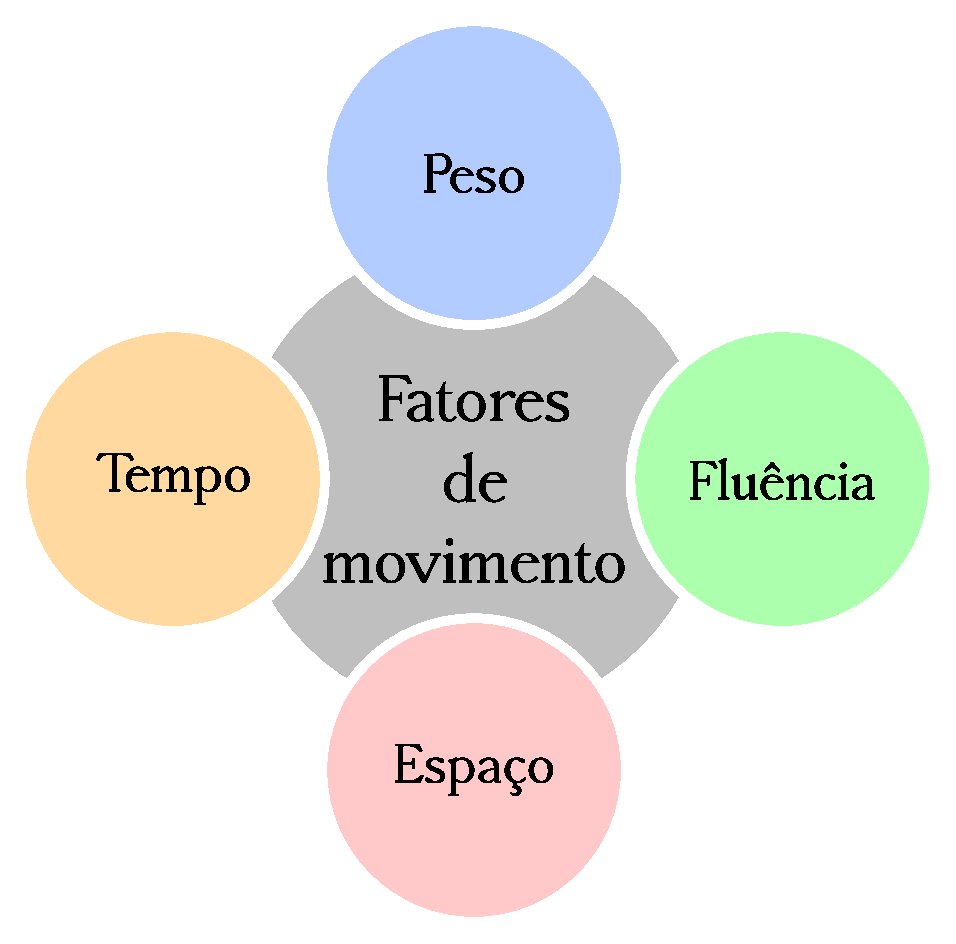
\includegraphics[width=0.4\textwidth]{chapters/cap-musicalidade/elementos-musica-1.eps}
\vspace{-5pt}
\caption{Fatores do movimento no modelo de Rudolf Laban.}
\vspace{-10pt}
\label{fig:fatores:moviemnto:Laban}
\end{wrapfigure}
A seguir vemos uma descrição detalhada de todos estes fatores:\\
\begin{description}
\item[Peso:]
Refere-se ao grau de tensão corporal para a execução de uma ação, 
a qual pode-se estar em algum ponto intermediário entre o firme e o leve 
(ou entre ``firm'' e ``fine'' em inglês) 
\cite[pp. 137, 143]{laban1987dominio}  \cite[pp. 5]{carline2011lesson} \cite[pp. 28]{elementosdanca2017}. 
\begin{itemize}
\item Firme: Os músculos estão tensionados, são uma fonte de resistência ao peso. Exemplos: O andar de um elefante, socos ou explodir.
\item Leve: Temos uma leve tensão muscular e um toque suave ou delicado,
tem uma leve resistência ao peso.  Exemplos: Ligeiro, flutuar.
\end{itemize}~
%%
\end{description}

\begin{description}
\item[Tempo:] Refere-se ao modo do uso do tempo no movimento,
onde pode-se estar em algum ponto intermediário entre o súbito e o sustentado 
(em inglês é conhecido como    ``sudden'' e ``sustained'') 
\cite[pp. 143]{laban1987dominio} \cite[pp. 5]{carline2011lesson} \cite[pp. 28]{elementosdanca2017}.
\begin{itemize}
\item Súbito: Envolve uma ação imediata e/ou surpreendente, é dizer de curta duração
ou com um sentir de momentaneidade. Exemplos: estancar-se numa posição, saltar.
\item Sustentado: O corpo leva um tempo para executar uma única ação, 
com um movimento persistente e contínuo, é dizer de duração indeterminada ou com um sentir interminável.  
Exemplos: Acomodar, afundar.
\end{itemize}~
\end{description}

\begin{description}
\item[Espaço:] Refere-se ao modo do deslocamento;
este pode estar em algum ponto intermediário entre  direto  e  flexível 
(em inglês é conhecido como  ``linear'' e ``curved'') 
\cite[pp. 143]{laban1987dominio} \cite[pp. 6]{carline2011lesson} \cite[pp. 28]{elementosdanca2017}.
\begin{itemize}
\item Linear: o movimento segue uma trajetória reta. Exemplo:
Um braço se estende de modo que a mão gere uma trajetória sobre uma linha,
com um sentir de estreiteza.
\item Curvado: O movimento tem movimentos realizando curvas ou torções,
com um sentir de movimentos manejáveis na sua extensão espacial. 
Exemplos: Um braço se estende de modo que a mão descreve uma meia lua e o antebraço realiza uma torção no seu eixo.
\end{itemize}~
%%
\item[Fluência :] (``flow'') Refere-se a quando nossos movimentos podem 
estar em algum ponto intermediário entre um movimento livre  e outro contido 
(em inglês é conhecido como   ``free'' e ``bound'')
\cite[pp. 140-143]{laban1987dominio} \cite[pp. 6]{carline2011lesson} \cite[pp. 27]{elementosdanca2017}.
\begin{itemize}
\item Livre: Quando o corpo se movimenta livremente num movimento continuo,
de modo que não existam emendas entre o final de um movimento e o inicio de outro.
\item Contido: Quando o movimento do corpo é interrompido,
de modo que é fácil distinguir como os movimentos estão estruturados em pedaços.
\end{itemize}~
\end{description}

%%%%%%%%%%%%%%%%%%%%%%%%%%%%%%%%%%%%%%%%%%%%%%%%%%%%%%%%%%%%%%%%%%%%%%%%%%%%%%%%
\subsection{Fatores de movimento: Um modelo atual}
\label{subsec:fator:movimento:atual}
\begin{wrapfigure}{r}{0.6\textwidth}
\centering
\smartdiagramset{
  text width=5.5cm,
  module minimum width=3.5cm,
  module minimum height=1.5cm
} 
\smartdiagram[bubble diagram]{Fatores do\\movimento,Força,Velocidade,Continuidade}
\caption{Fatores do movimento comumente usados.}
\label{fig:fatores:moviemnto:popular}
\end{wrapfigure}
Atualmente (\AnoLivro), muitos profissionais do mundo da dança, 
 acostumam usar modelos pedagógicos, 
com outras subdivisões diferentes aos fatores do movimento descritos por Laban; 
porém estes modelos também separam as dinâmicas dos movimentos em fatores;
por exemplo, é comum achar o modelo  mostrado na Figura \ref{fig:fatores:moviemnto:popular},
na literatura \cite[pp. 30]{paine2014complete} \cite[pp. 181]{smith2014dance}
e em meios audiovisuais que abordam temas relativos a dança:

\begin{description}
\item[Força:] (Suave $\rightarrow$ forte) 
É relativo à intensidade da força que usamos ao realizar nossos movimentos;
onde podemos escolher níveis de forças em algum ponto intermediário entre suave e forte. 
\end{description}

\begin{description}
\item[Velocidade:] (Lento $\rightarrow$ rápido)
Se refere à velocidade ao executar nossos movimentos;
onde podemos escolher velocidades em algum ponto intermediário entre lento e rápido. 
\item[Continuidade:] (Continuo $\rightarrow$ abrupto)
Refere-se ao grau de continuidade ao realizar nossos movimentos;
onde podemos escolher valores de continuidade em algum ponto intermediário entre continuo e abrupto.
\end{description}
Seja qual for a notação que usemos, sempre poderemos ordená-los em escalas
que tem dois extremos e infinitos pontos intermediários,
como é mostrado na Figura \ref{fig:element:moviment},
onde vemos como podemos realizar cada movimento selecionando umas caraterísticas especificas de força (F), velocidade (V) e continuidade (C);
é dizer com uma dinâmica (D),  $D=\{F, V, C\}$.
\begin{figure}[!h]
\centering
    \begin{subfigure}[b]{0.45\textwidth}
    \centering
    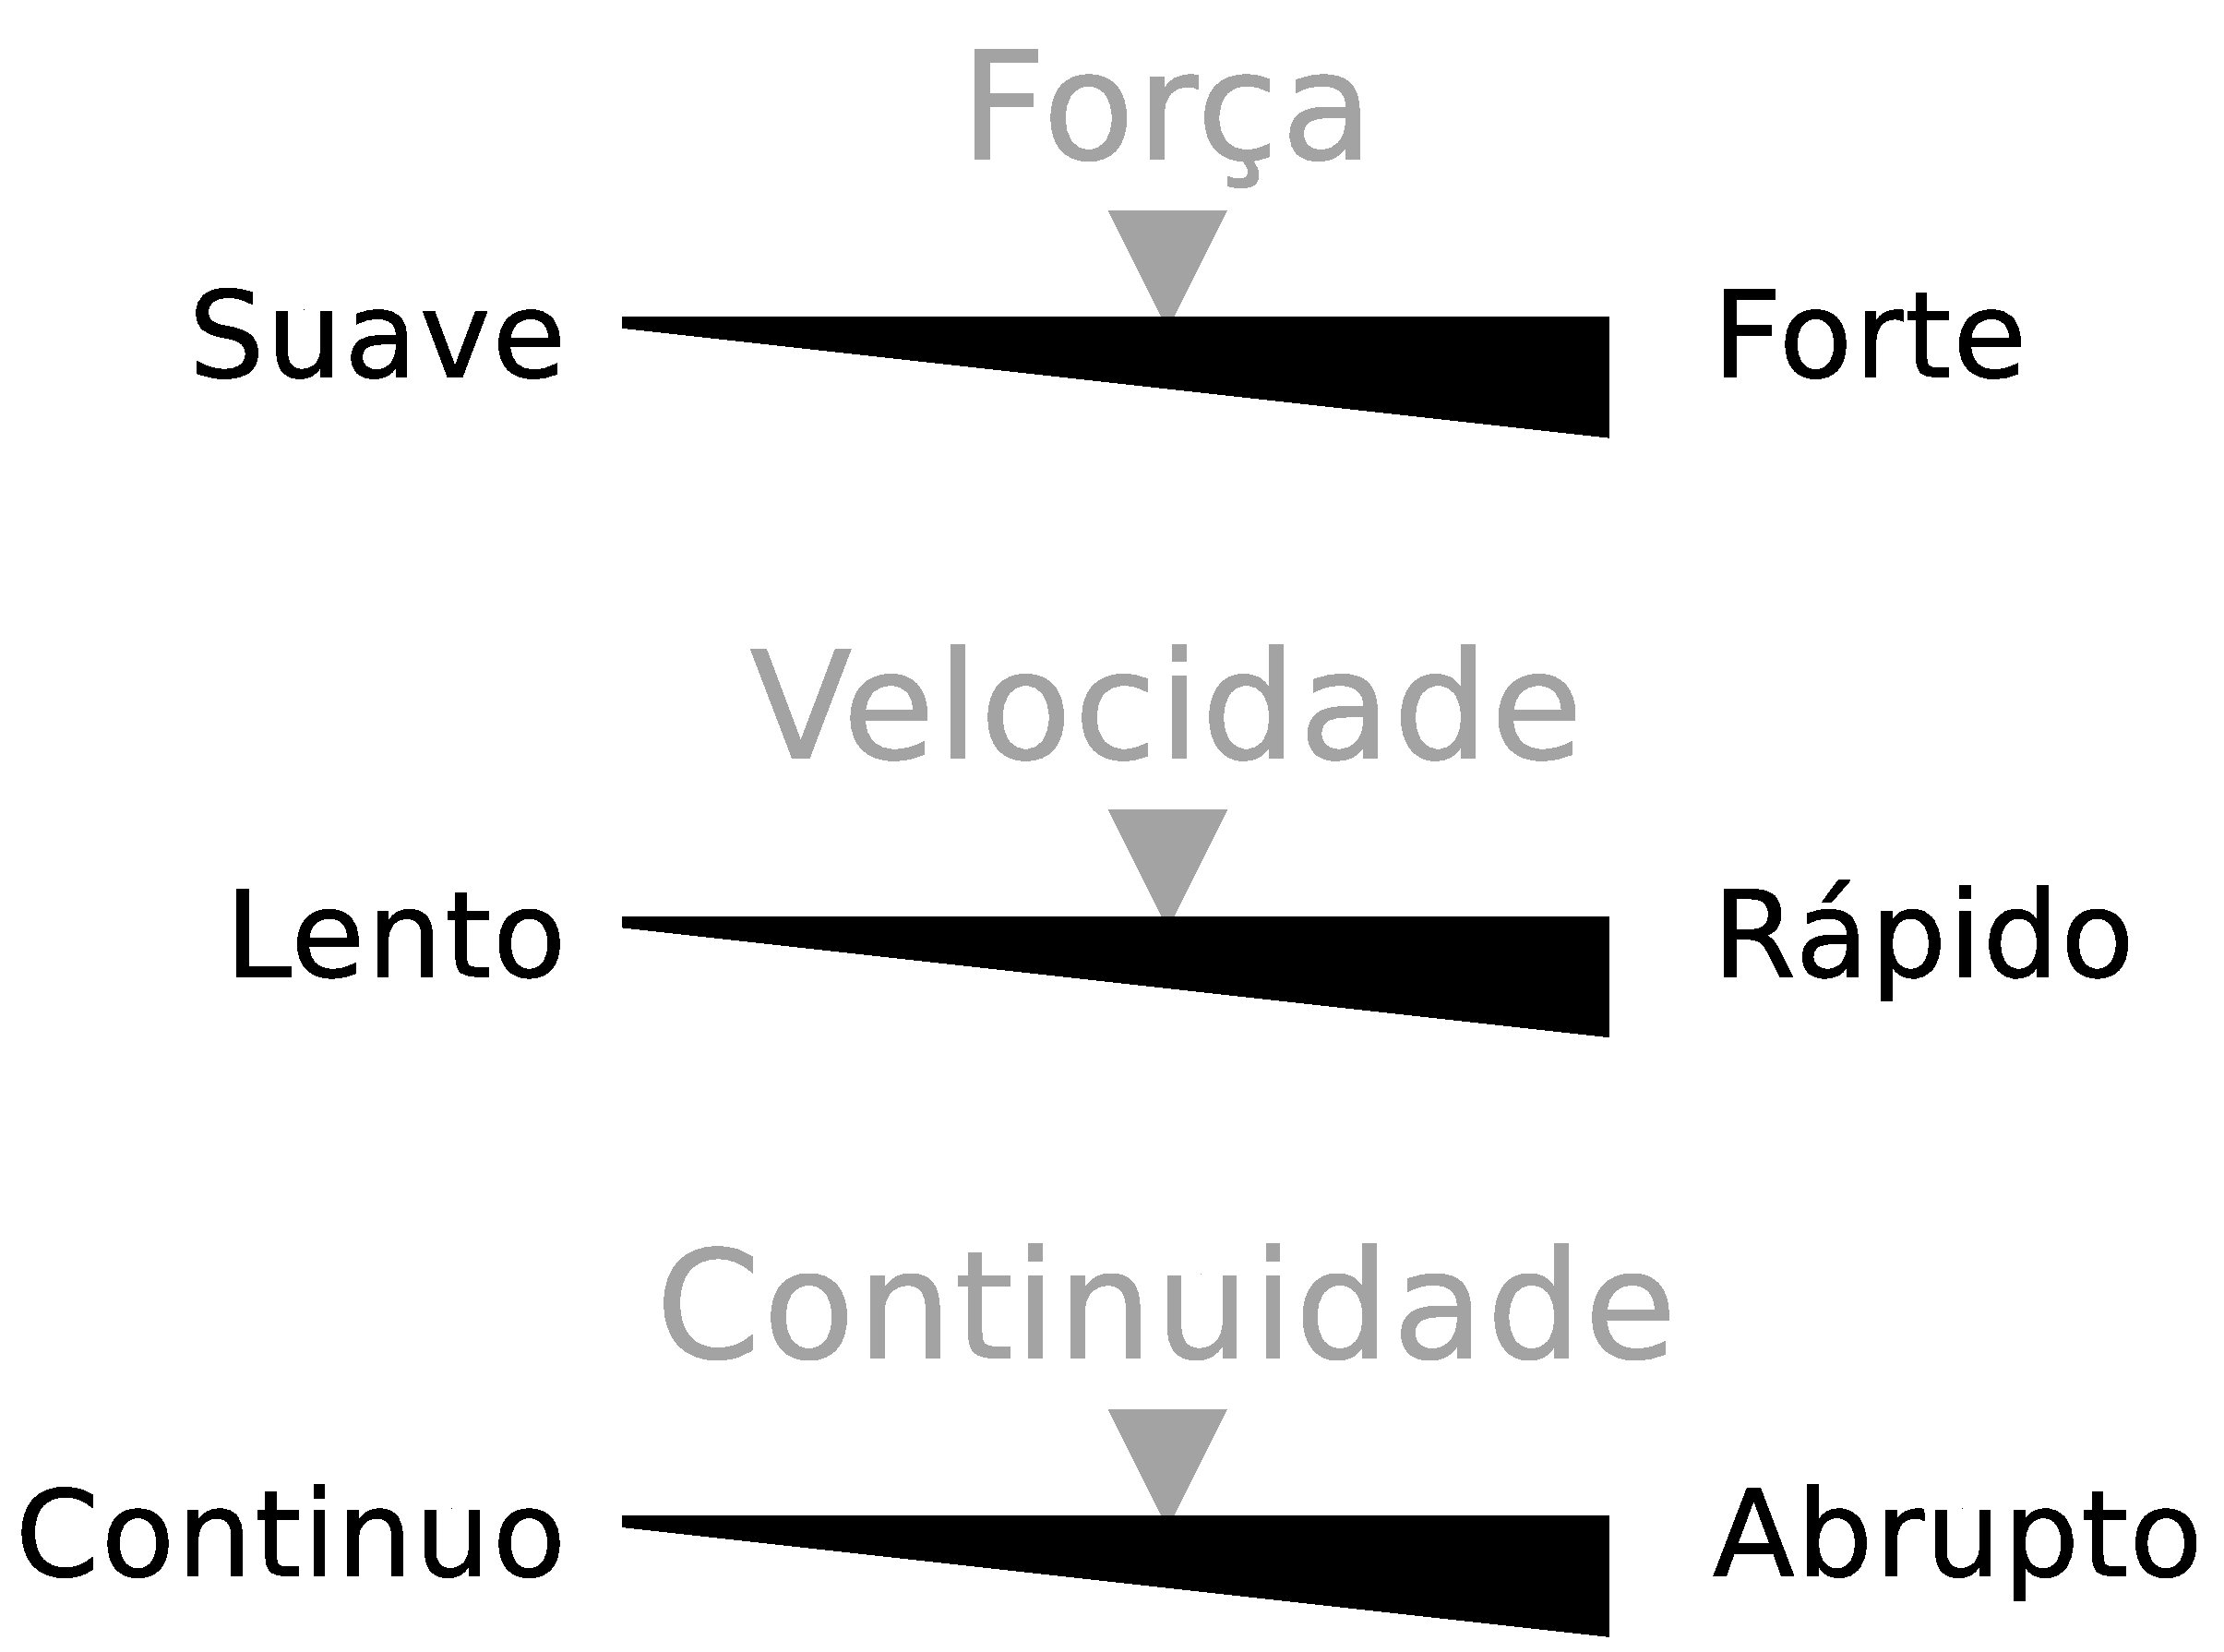
\includegraphics[width=0.95\textwidth]{chapters/cap-musicalidade/dinamicas-elementos1.eps}
    \caption{Caraterísticas do movimento.}
    \label{fig:element:moviment}
    \end{subfigure}
    \hfill
    \begin{subfigure}[b]{0.5\textwidth}
    \centering
    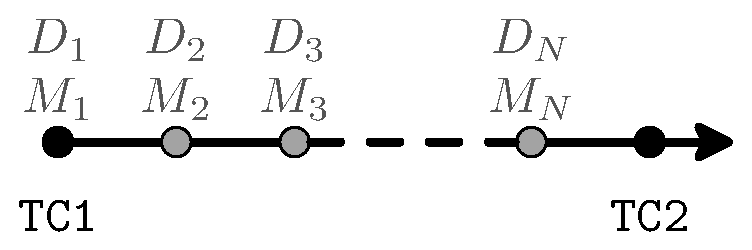
\includegraphics[width=0.95\textwidth]{chapters/cap-musicalidade/dinamicas-elementos1b.eps}
    \caption{Movimentos entre tempos coreográficos.}
    \label{fig:coreografia:moviment}
    \end{subfigure}
\caption{Dinâmicas dos movimentos.}
\label{fig:geral:moviment}
\end{figure}
Assim, podemos definir que entre dois \hyperref[sec:TemposCoreograficos]{\textbf{tempos coreográficos}} consecutivos,
podemos realizar coreografias com $N$ movimentos $M_n$, com $n=\{1, 2, ..., N\}$, 
de modo que a cada um destes movimentos lhe corresponda uma dinâmica $D_n=\{F_n, V_n, C_n\}$,
como pode ser visto na Figura \ref{fig:coreografia:moviment}.
\begin{example}[Explorando força e velocidade:]
Podemos estudar as dinâmicas de nossos movimentos fazendo um pequeno exercício,
primeiro escolheremos um movimento (M1), por exemplo: estirar os braços.
e depois usaremos 4 diferentes dinâmicas para executar-lho,
levando ao extremo as caraterísticas de força e velocidade,
e deixando num valor intermediário a continuidade.
Estas escolhas podem ser facilmente visualizadas na Figura \ref{fig:element:moviment2}.
\end{example}


\begin{figure}[!h]
  \centering
    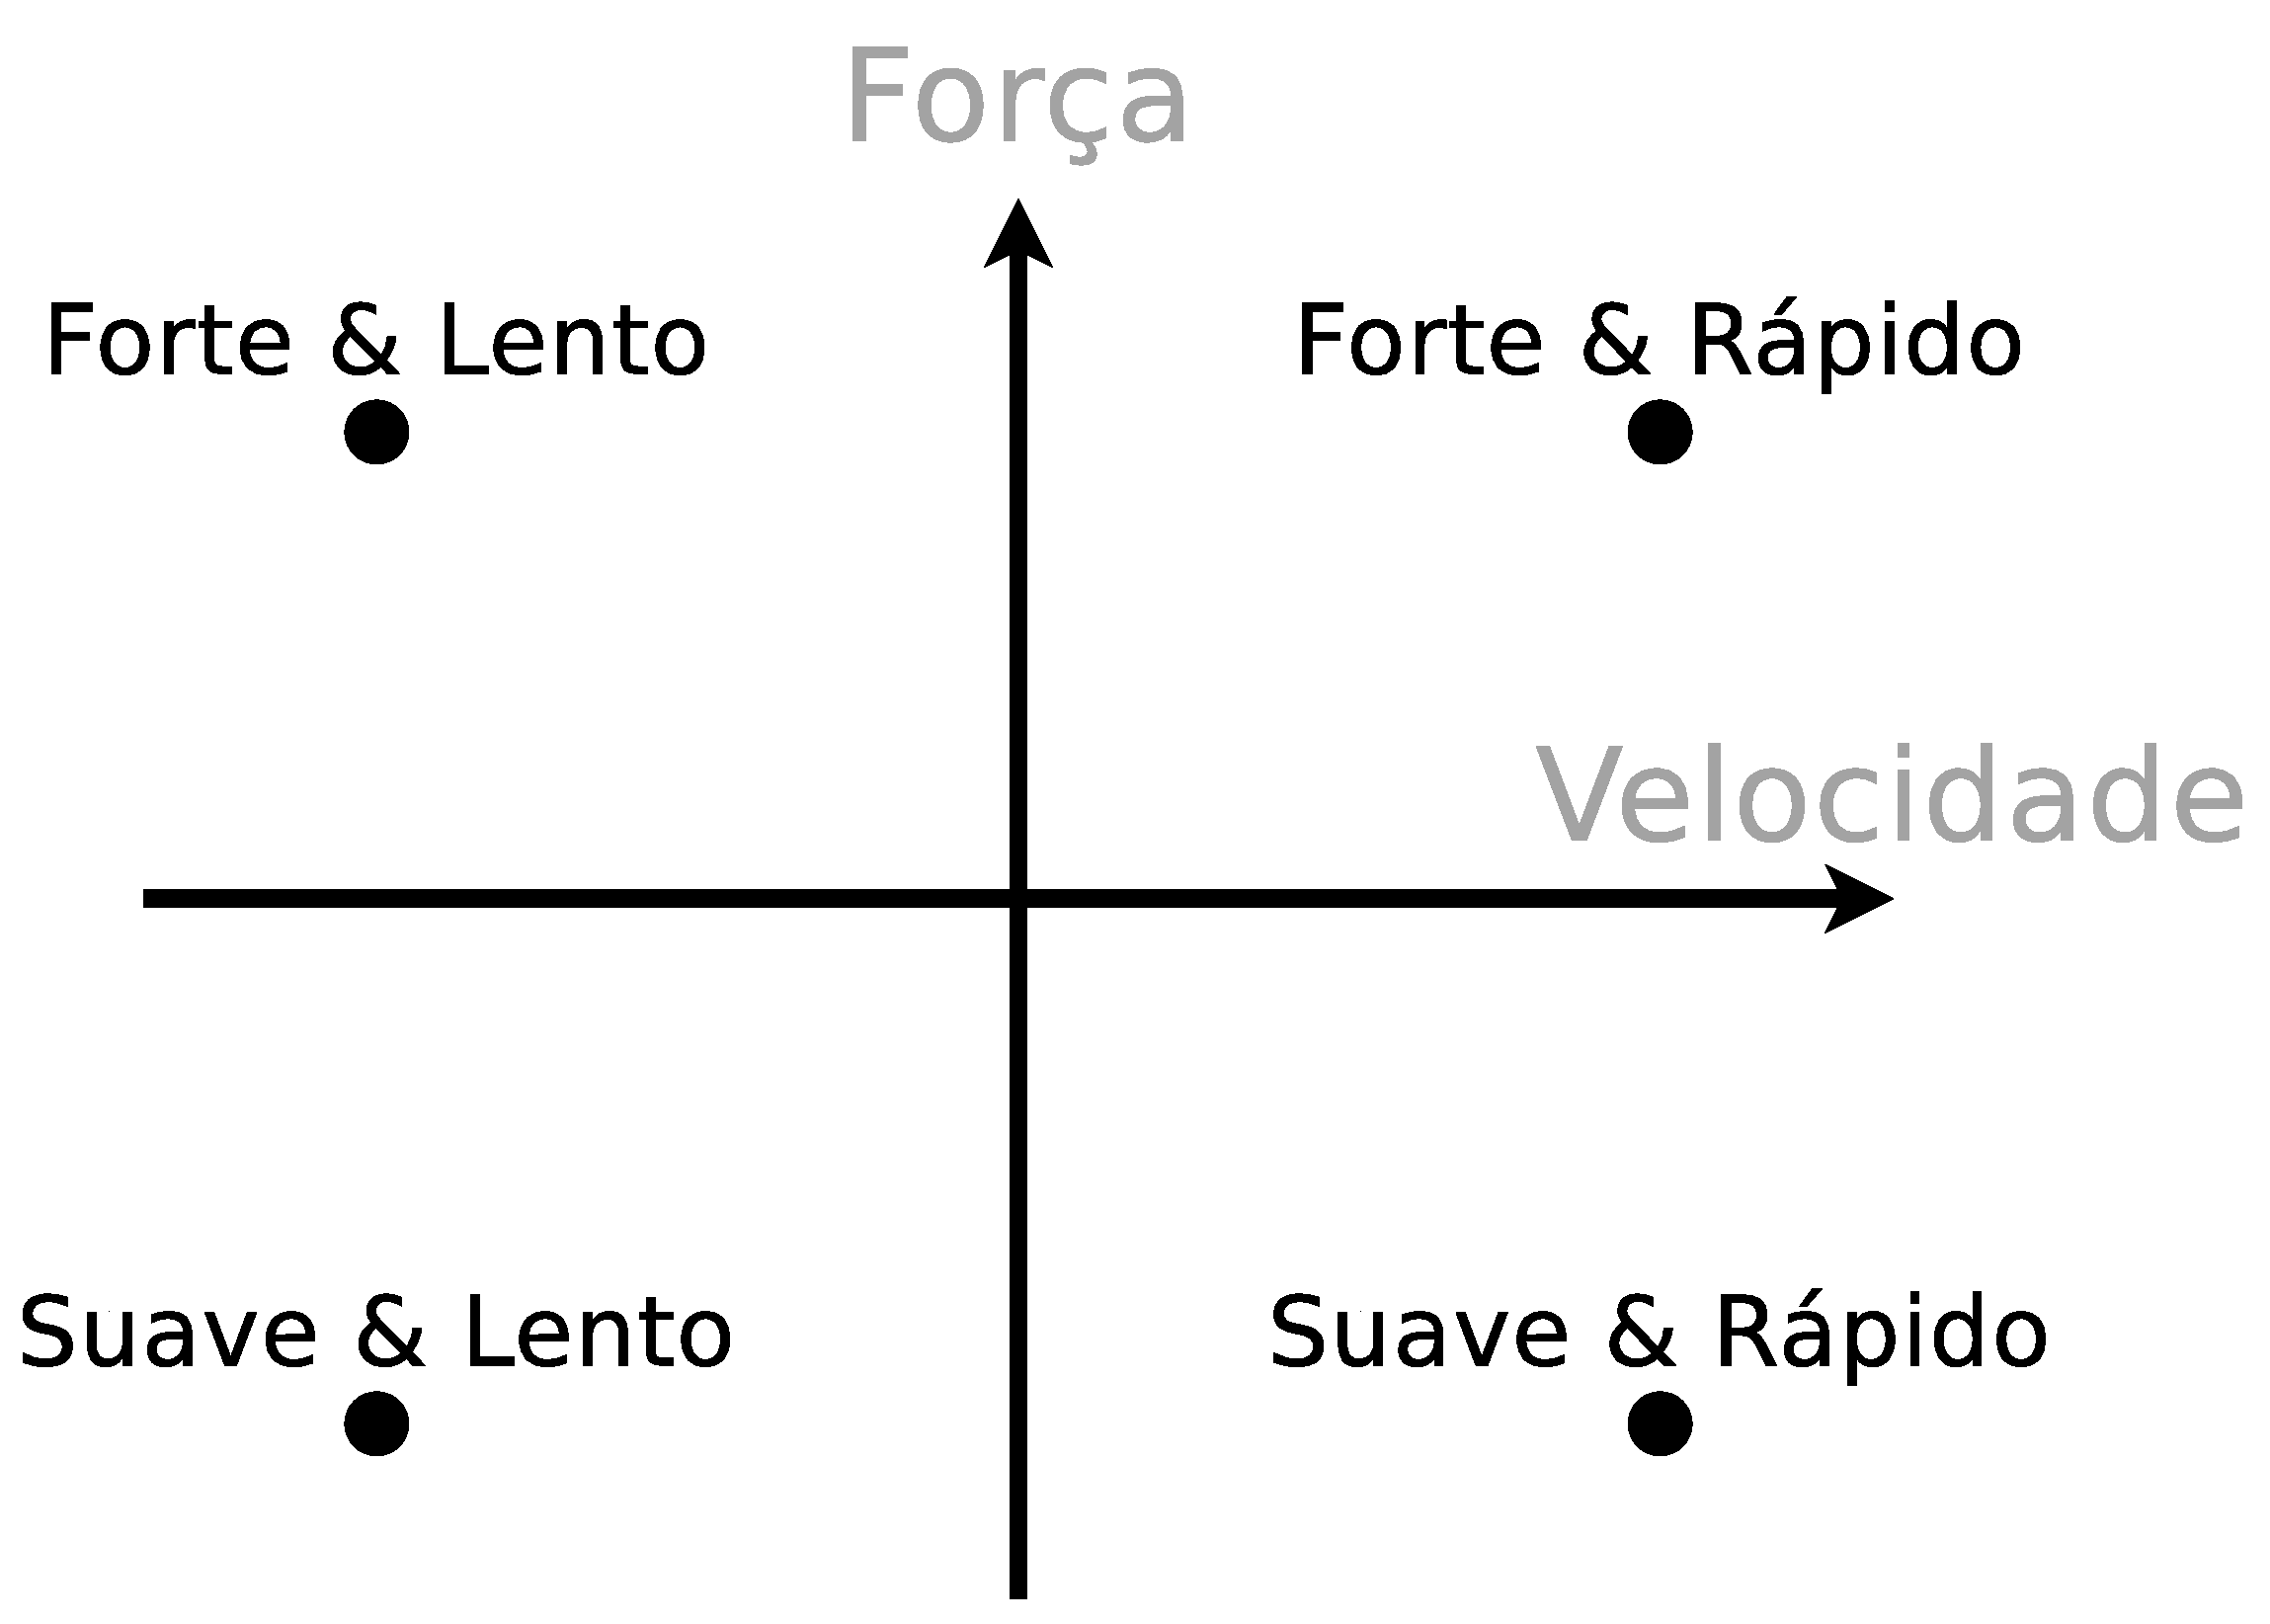
\includegraphics[width=0.45\textwidth]{chapters/cap-musicalidade/dinamicas-elementos2.eps}
\caption{Combinando elementos.}
\label{fig:element:moviment2}
\end{figure}

\begin{example}[Treino de ``Lady style'':]
\index{Lady style}
No treinamento de enfeites femininos (também conhecido como ``lady style'')
é possível observar a importância do uso das dinâmicas;
por exemplo, se escolhemos um movimento, 
como levantar os braços e logo descer eles (como quando o seguidor faz um giro).
Podemos observar uma variedade de texturas do movimento,
modificando os parâmetros  \{F,V,C\} nas dinâmicas.
\begin{itemize}
\item Os braços podem subir e descer fazendo um movimento continuo, leve e lento.
\item Os braços podem subir num movimento forte e rápido,
e com uma transição continua descer os braços de forma leve e lenta.
\item Os braços podem subir leve e lento,
e com uma transição continua descer os braços com tensão muscular e rápida 
(explosivo com arrumada ou desarrumada de cabelo). 
\item Etc.
\end{itemize}
\end{example}

%%%%%%%%%%%%%%%%%%%%%%%%%%%%%%%%%%%%%%%%%%%%%%%%%%%%%%%%%%%%%%%%%%%%%%%%%%%%%%%%
\subsection{Fatores do movimento: Um modelo simplificado}

\begin{wrapfigure}{r}{0.6\textwidth}
\centering
\begin{comment}
\smartdiagramset{
  text width=5.5cm,
  module minimum width=3.5cm,
  module minimum height=1.5cm
} 
\smartdiagram[bubble diagram]{Fatores do\\movimento,Energia,Continuidade}
\end{comment}
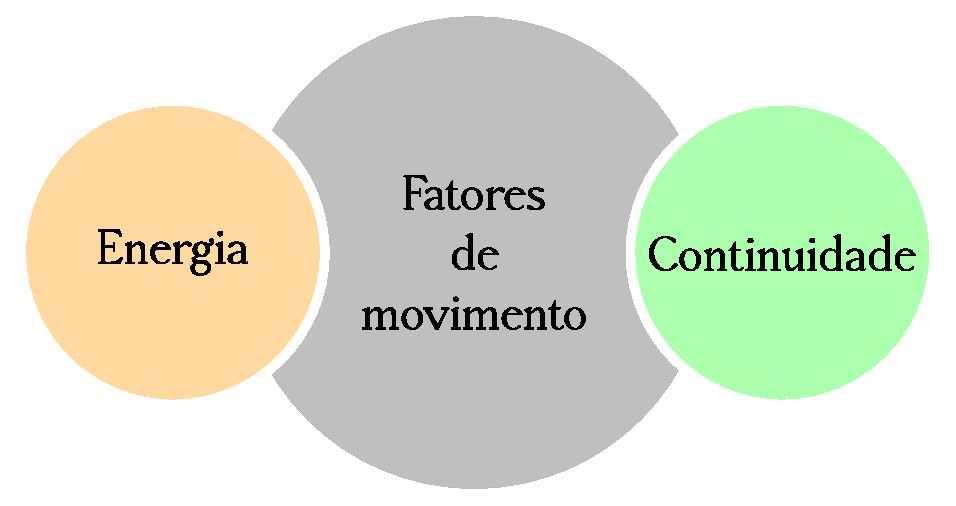
\includegraphics[width=0.55\textwidth]{chapters/cap-musicalidade/fatores-de-movimento.eps}
\caption{Fatores do movimento num modelo simplificado.}
\label{fig:fatores:moviemnto:simplificada}
\end{wrapfigure}
Seguindo alguns profissionais  da dança, 
as dinâmicas do movimento nos indicam a forma em que a energia do corpo
é gastada, liberada ou modulada na dança \cite[pp. 126, 131, 136]{mccutchen2006teaching}.

Podemos usar a energia em vários níveis de intensidade ou estágios,
sendo que o uso da energia envolve também o uso de vários níveis de intensidade 
nos fatores velocidade e força, vistos na Seção  \ref{subsec:fator:movimento:atual} \cite[pp. 99]{sofras2019dance}.

Seguindo o coreografo e dançarino, Alonzo King \cite[pp. 99, 100]{sofras2019dance}:
\begin{citando}%%
Energia é a textura entre os movimentos.
Os movimentos falam com os dançarinos.
Estados físicos criam estados emocionais.
\end{citando}
Alonzo também indica que a energia usada nos movimentos,
 cria frases de dança com significado e dimensão \cite[pp. 99]{sofras2019dance}.

A energia pode ser usada para contrair ou tensionar os músculos,
movimentar-nos rapidamente ou lenta e controladamente, pular, 
ou para conter e segurar nossa inercia gerando uma mudança abruta no fluxo da energia.

Assim, 
uma forma muito simplificada de iniciar as pessoas a trabalhar no uso das dinâmicas do movimento,
é separando as nossas dinâmicas em dois fatores:
\begin{description}
\item[Energia] (Baixo nível de energia $\rightarrow$ Alto nível energia)
Refere-se a quantidade de energia que gastamos em realizar nosso movimento;
este pode estar em algum ponto intermediário entre dois níveis de energia. 
O uso da energia, como fator de movimento, embrulha num só fator os 
fatores velocidade e força vistos na Seção  \ref{subsec:fator:movimento:atual}.
\item[Continuidade:] (Continuo $\rightarrow$ abrupto)
Este fator de movimento é o mesmo que vimos na Seção \ref{subsec:fator:movimento:atual};
refere-se ao grau de continuidade ao realizar nossos movimentos;
onde podemos escolher valores de continuidade em algum ponto intermediário entre continuo e abrupto.
\end{description}~

\begin{example}[Explorando o uso de níveis de energia:]
Podemos estudar a energia de nossos movimentos fazendo um pequeno exercício,
primeiro escolheremos um movimento, por exemplo: estirar os braços.
e depois usaremos 3 diferentes níveis de energia para executar este movimento;
por exemplo: baixa, meio ou alto nível de energia.
\end{example}

%%%%%%%%%%%%%%%%%%%%%%%%%%%%%%%%%%%%%%%%%%%%%%%%%%%%%%%%%%%%%%%%%%%%%%%%%%%%%%%%
\subsection{Dinâmica: Força - Tensão e Relaxação }
\label{sec:musicalidadetensionrelease}

% Bryan Adams - Summer Of '69 
%https://tabs.ultimate-guitar.com/tab/bryan_adams/summer_of_69_chords_843137

% https://books.google.com.br/books?id=PZdnDTxLscIC&pg=PA7&lpg=PA7&dq=tension+%2B+release+%2B+dance&source=bl&ots=c42uHzTXla&sig=ACfU3U1lZmDB5Jd23e41icQQKpzUnea0nw&hl=pt-BR&sa=X&ved=2ahUKEwj2-qz4ha3kAhUsIbkGHdRyBQgQ6AEwEnoECAgQAQ#v=onepage&q=tension%20%2B%20release%20%2B%20dance&f=false

Como vimos nas seções anteriores,
um dos fatores do movimento é a ``força'', 
ou o ``peso'' no modelo de Laban,
sendo que este fator pode ter valores entre dois extremos,
que nesta seção chamaremos como, ``relaxação'' e ``tensão''.
Este fator é muito usado, 
devido a que nós controlamos nossos movimentos corporais 
mediante um balance entre a tensão e a relaxação muscular \cite[pp. 7]{schrader2005sense}.

Quando queremos explorar o fator força em nossa dança, tentaremos na medida do possível,
manter os outros fatores como velocidade e continuidade em valores intermediários,
para que o protagonismo no movimento seja para o fator força,
que será usado modificando seu valor desde a relaxação até a tensão, e vice-versa, no transcurso dos movimentos. 

Como vimos na Seção \ref{sec:tensionrelease}, 
ao escutar música comumente percebemos ciclos de tensão e relaxação,
provocadas por dissonâncias,  cadências nas frases musicais, ou mudanças de
tom, intensidade, ritmo, etc.
Assim, 
seguindo o explicado sobre o \hyperref[sec:interpretacioncorporal]{\textbf{mapeamento}}\footnote{Para
ver o tema do mapeamento de aspectos da música ir a Seção \ref{sec:interpretacioncorporal}.} 
de aspectos da música e aspectos do movimento,
podemos associar a tensão e relaxação dos movimentos de nossa dança à música.



\begin{description}
\item[Tensão muscular:] Para gerar tensão, 
deveremos realizar nossos movimentos aumentado o grau de ativação muscular (contração muscular, aspecto de potencia), 
seguindo nossa imaginação e  critério;
para projetar uma imagem, por exemplo, de que estamos suportando tensão (como quando puxado por uma corda), 
peso (como um andar carregando um objeto pesado), força (como empurrando um objeto pesado), etc.
Para mais detalhes sobre ativação muscular ver os  Exemplos \ref{ex:tension:on}, \ref{ex:tension:on2} e \ref{ex:tension:on3}.
\begin{example}[Ativação muscular no esforço:]
\label{ex:tension:on}
Imaginemos que debemos mexer nossa mão 30 cm a direita, em 3 segundos;
porém, na primeira tentativa, nos temos que arrastrar com essa mão um pacote de 5Kg,
e na segunda vez não.
É evidente que, tendo em ambos casos a mesma velocidade e percorrido,
no primeiro a nossa ativação muscular será superior que no segundo caso.
\end{example}
\begin{example}[Ativação muscular do carateca:]
\label{ex:tension:on2}
Imaginemos a um carateca realizando seus treinamentos de forma unipessoal, 
fazendo sombra; é dizer, lutando com um oponente imaginário;
nesse instante mesmo sem fazer contato físico com seu adversário,
ele está com uma elevada ativação muscular em cada golpe,
sendo esta caraterística evidente para qualquer  observador.
\end{example}
\begin{example}[Ativação muscular do mimo:]
\label{ex:tension:on3}
Outra forma de ver ativação muscular é quando assistimos a apresentação de um mimo,
e ele faz os movimento de  abrir uma porta e carregar ou empurrar um objeto;
não só reproduzindo a trajetória dos movimentos, 
se não que também incorporando a ativação muscular necessária que teria o movimento. 
\end{example}
\item[Relaxação muscular:] Para gerar relaxação, 
deveremos realizar nossos movimentos, 
de modo que seja  perceptível para nós um movimento predominantemente ósseo\footnote{Esta
descrição é para estar no extremo da relaxação.}, 
que um movimento por ativação muscular;
é evidente que todo movimento tem ativação muscular,
porém na relaxação esta caraterística não é o protagonista,
e sim o movimento ósseo.
\begin{example}[Relaxação da marionete:]
Imaginemos uma marionete controlada por fios, 
onde podemos observar o movimento relaxado do boneco.
A marionete se movimenta sem ativação muscular, 
e só percebemos nele o movimento ósseo de suas extremidades, 
contido só pelas suas articulações.

Assim, a maneira de treinamento, 
podemos tentar movimenta-nos imitando os movimentos de uma marionete,
para poder entender como é um corpo com relaxação extrema,
e como incorporar esta caraterística dosificadamente em nossos movimentos de dança.
\end{example} 
\end{description}

~

\PRLsep{Break aplicando tensão e relaxação}
\index{Musicalidade!Break}

Uma forma de aproveitar os \hyperref[sec:UsandoBreak]{\textbf{breaks}} na música,
é criando dinâmicas de tensão e relaxação.
Isto é, criar tensão  no nosso corpo quando o break está a ponto de estourar,
e relaxação no silencio provocado quando o break estourou,
como é mostrado na Figura \ref{fig:tension-release-climax}.
O quanto tempo usemos para acumular tensão e para liberar-lha 
é uma escolha criativa de cada um, 
limitado unicamente pelo tempo que disponhamos;
por exemplo, o tempo de silencio num break geralmente é curto.



\begin{figure}[!h]
  \centering
    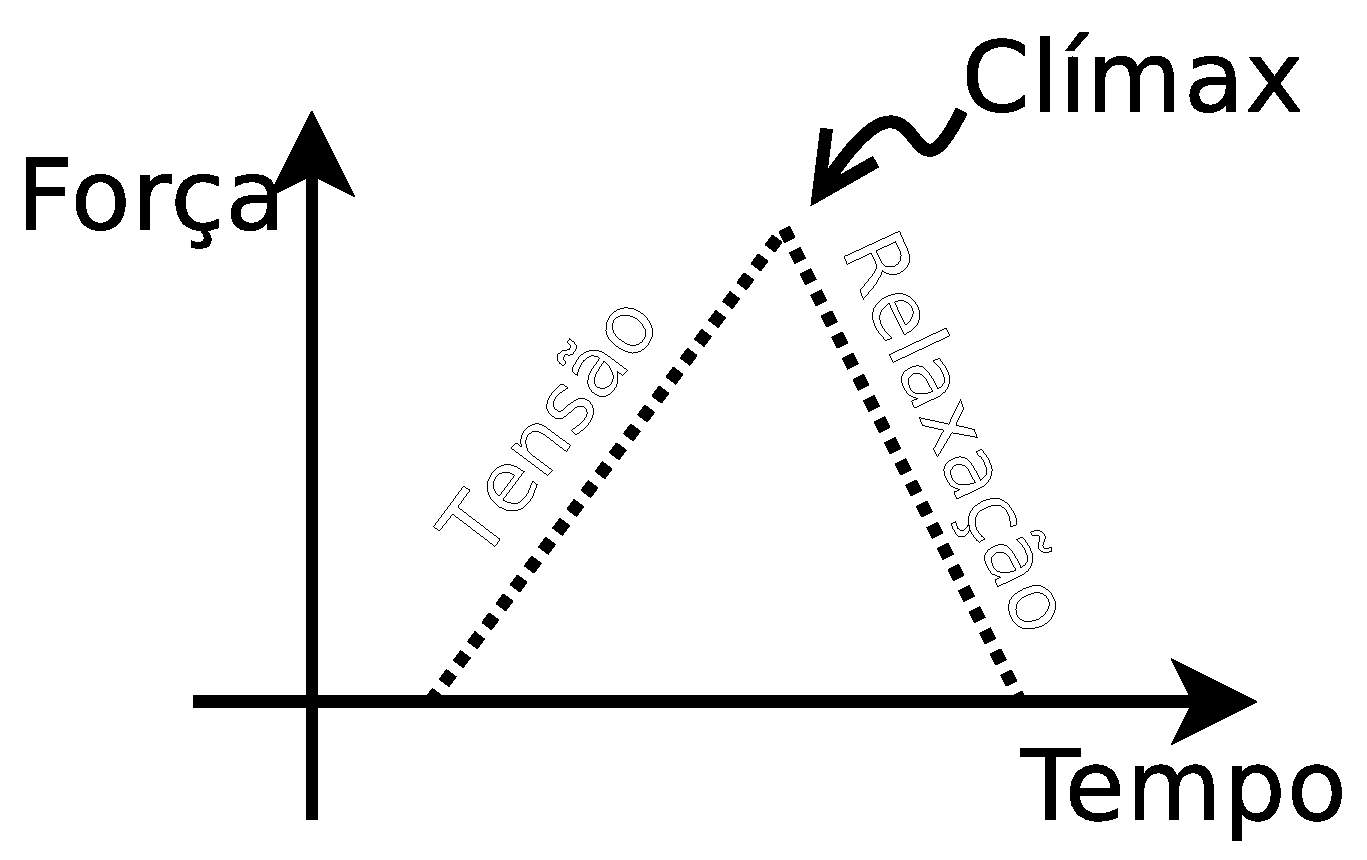
\includegraphics[width=0.5\textwidth]{chapters/cap-musicalidade/tension-release-climax.eps}
\caption{Uso do \hyperref[ref:climax]{\textbf{clímax}} na dinâmica de tensão e relaxação.}
\label{fig:tension-release-climax}
\end{figure}


\PRLsep{Dança a dois aplicando tensão e relaxação}

Podemos aproveitar a dinâmica da tensão e relaxação na dança a dois,
já seja de forma unipessoal ou como trabalho de par,
a continuação são listadas algumas dicas.
\begin{itemize}
\item Se o condutor está com um abraço fechado de dança, 
é possível aproveitar a mudança de tensão a relaxação da música,
criando tensão muscular nosso último movimento antes do \hyperref[ref:climax]{\textbf{clímax}} na música,
para logo paulatinamente voltar a uma relaxação muscular,
dando um efeito de mola que estica e encolhe,
para qualquer de nossos movimentos.
\item Se estamos com um abraço de dança aberto, ou estamos dançando separados de nosso par,
qualquer pessoa do par de dança pode aplicar a tensão e relaxação muscular, 
no seu próprio corpo de maneira independente, possivelmente gerando uma posse,
e voltando a relaxação, ou estendendo o último movimento realizado na dança,
em qualquer caso o efeito visual será parecido a uma mola que se tensiona e logo se relaxa.
\end{itemize}



%%%%%%%%%%%%%%%%%%%%%%%%%%%%%%%%%%%%%%%%%%%%%%%%%%%%%%%%%%%%%%%%%%%%%%%%%%%%%%%%
%https://translate.google.com.br/translate?sl=en&tl=pt&u=https%3A%2F%2Fblog.steezy.co%2Fwhat-are-textures-in-dancing%2F
\subsection{Dinâmica: Continuidade - Legato e sttacato}
\label{subsec:continuidade:ls}
\index{Musicalidade!Articulação}
\index{Musicalidade!Continuidade}
\index{Musicalidade!Legato}
\index{Musicalidade!Sttacato}


O fator do movimento ``continuidade'', 
ou ``flow'' em inglês, tem valores entre dois extremos: continuo e  abrupto.
Na maioria das vesses quando dançamos estamos num valor intermédio de continuidade,
sem aproveitar demasiado os extremos.
Assim, quando desejamos explorar este fator, manteremos na medida do possível,
os outros fatores como velocidade e força em valores intermediários,
para assim poder ressaltar a continuidade.

Como vimos na Seção \ref{sub:Articulation}, 
ao escutar uma música percebemos que existem formas de \hyperref[sub:Articulation]{\textbf{articular}} as notas musicais;
por exemplo, estas podem ser articuladas em 
\hyperref[subsec:Legato]{\textbf{legato}} ou \hyperref[subsec:Staccato]{\textbf{staccato}};
e dizer, as notas podem ser executadas consecutivamente sem emendas ou 
estas podem ser executadas de modo que seja claro onde inicia uma nota musical e onde termina a outra.
Assim, 
seguindo o explicado sobre o \hyperref[sec:interpretacioncorporal]{\textbf{mapeamento}}\footnote{Para
ver o tema do mapeamento de aspectos da música ir a Seção \ref{sec:interpretacioncorporal}.} 
de aspectos da música e aspectos do movimento,
podemos associar as articulações da música à dinâmica de continuidade nos movimentos de nossa dança.\\


\begin{description}
\item[Continuo:] Para gerar continuidade em nossos movimentos,
estes não devem ter emendas nem pausas; 
podem existir claro mudanças de velocidade e direção,
porém estas devem ser graduais e sutis.
\begin{example} 
Na Figura \ref{fig:continudade-all} temos umas curvas que representam uma metáfora de nossos movimentos,
onde os círculos indicam o inicio de cada movimento.
\begin{itemize}
\item Na Figura \ref{fig:continudade-a} vemos movimentos que são realizados de forma continua, 
em toda extensão destes, 
e inclusive a continuidade se conserva quando passamos de um tipo de movimento a outro.
\item Na Figura \ref{fig:continudade-b} vemos movimentos que são realizados de forma continua, 
em toda extensão destes;
porém a  continuidade se perde quando passamos de um tipo de movimento a outro.
\item Na Figura \ref{fig:continudade-c} vemos movimentos que são realizados de forma continua e linear,
diretos e sem movimentos desnecessários em toda extensão destes;
a continuidade é perdida quando passamos de um tipo de movimento a outro.
\end{itemize}
\end{example}

\item[Abrupto:] Para gerar descontinuidade em nossos movimentos, 
podemos eles realizando mudanças abruptas de direção, velocidade ou força,
de modo que seja evidente para qualquer observador cada tramo de nossos movimentos.
\begin{example}
Na Figura \ref{fig:continudade-all} temos umas curvas que representam uma metáfora de nossos movimentos,
onde os círculos indicam o inicio de cada movimento.
\begin{itemize}
\item Na Figura \ref{fig:continudade-d} vemos movimentos que são realizados de forma abrupta ou descontinua,
em toda extensão destes, 
e inclusive quando passamos de um tipo de movimento a outro.
\item Nas Figuras \ref{fig:continudade-b} e \ref{fig:continudade-c} 
vemos movimentos que só são descontínuos e abruptos nas emendas entre movimentos. 
\end{itemize}
\end{example}
\end{description}

\begin{figure}[!h]
     \centering
     \begin{subfigure}[b]{0.35\textwidth}
         \centering
         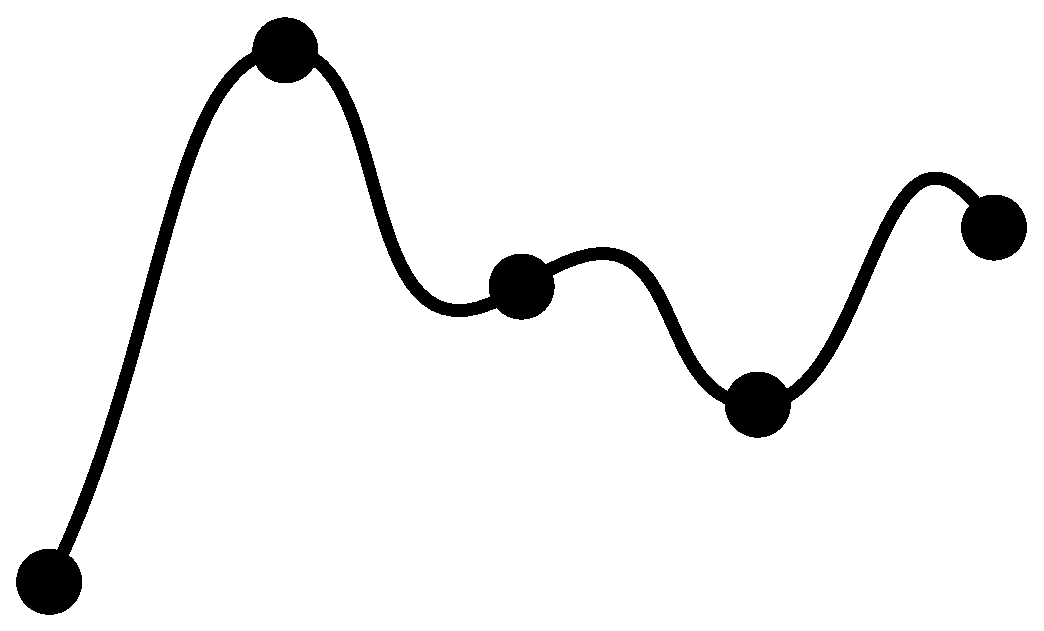
\includegraphics[width=0.8\textwidth]{chapters/cap-musicalidade/continudade-a.eps}
         \caption{Continuo no percorrido e emendas.}
         \label{fig:continudade-a}
     \end{subfigure}
     \hfill
     \begin{subfigure}[b]{0.35\textwidth}
         \centering
         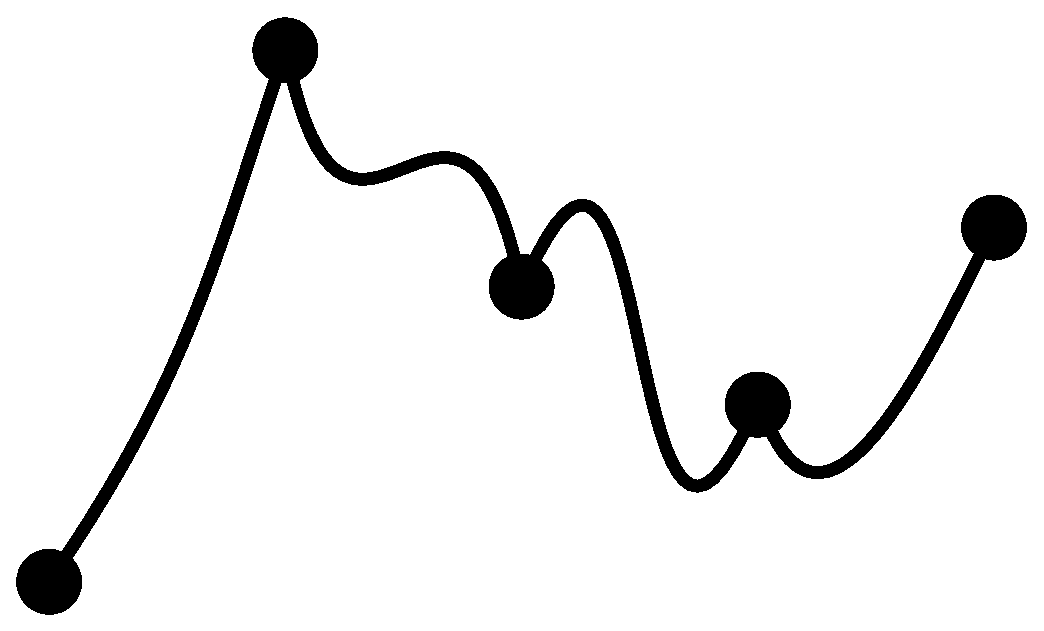
\includegraphics[width=0.8\textwidth]{chapters/cap-musicalidade/continudade-b.eps}
         \caption{Continuo no percorrido e abrupto nas emendas.}
         \label{fig:continudade-b}
     \end{subfigure}
     \hfill
     \begin{subfigure}[b]{0.35\textwidth}
         \centering
         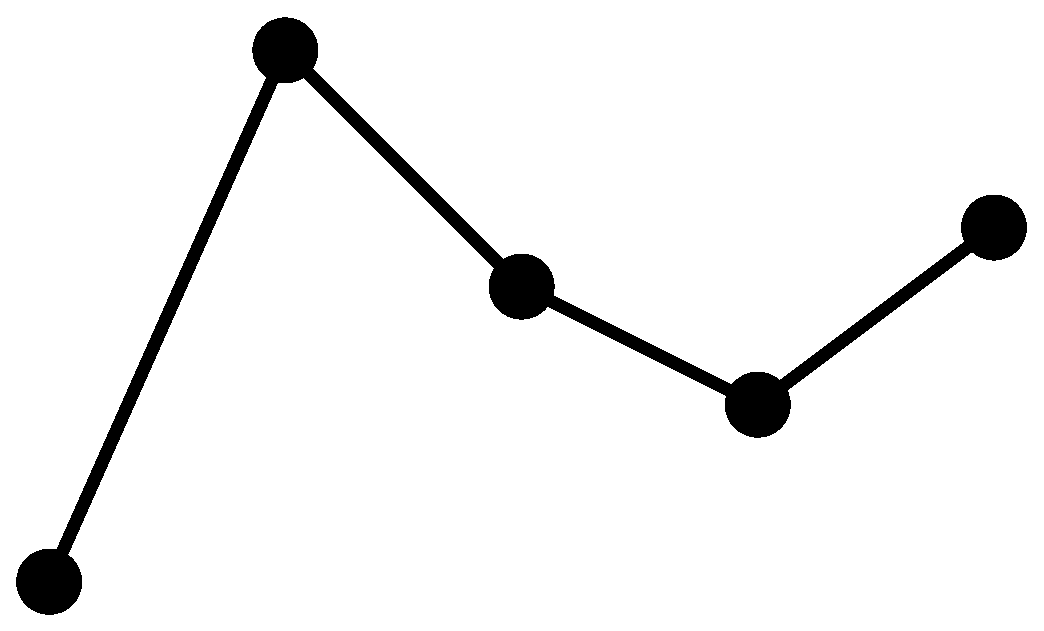
\includegraphics[width=0.8\textwidth]{chapters/cap-musicalidade/continudade-c.eps}
         \caption{Continuo linear no percorrido e abrupto nas emendas.}
         \label{fig:continudade-c}
     \end{subfigure}
     \hfill
     \begin{subfigure}[b]{0.35\textwidth}
         \centering
         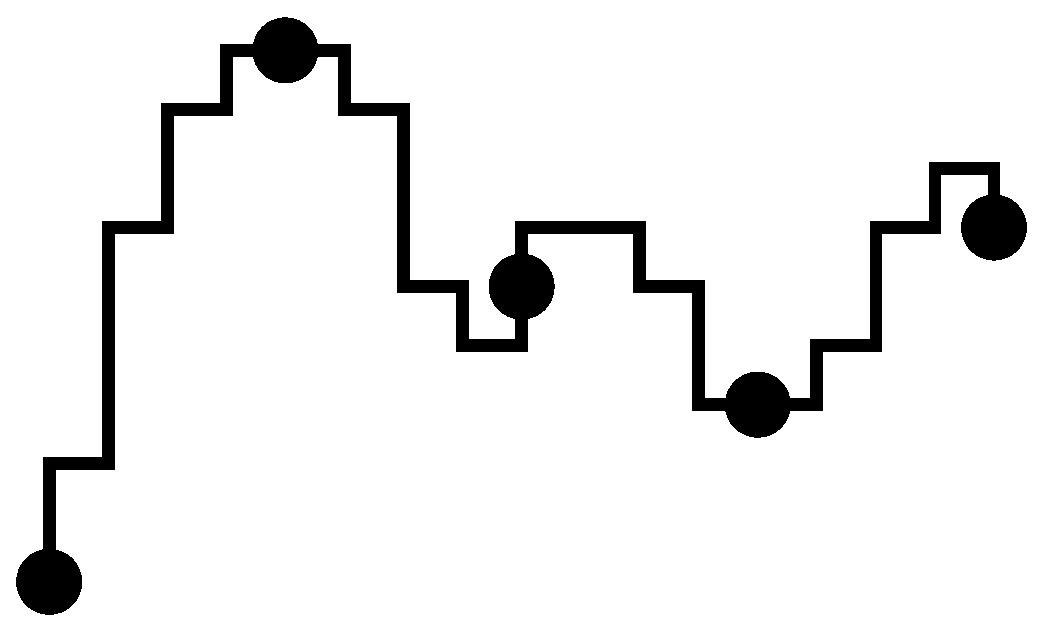
\includegraphics[width=0.8\textwidth]{chapters/cap-musicalidade/continudade-d.eps}
         \caption{Abrupto no percorrido e emendas.}
         \label{fig:continudade-d}
     \end{subfigure}
\caption{Usos do fator de movimento: continuidade.}
\label{fig:continudade-all}
\end{figure}

\begin{example}[Samba funkeado:]
Um exemplo interessante de movimentos abruptos nas emendas, 
é no estilo de dança \hyperref[subsec:sambafunkeado]{\textbf{samba funkeado}},
onde os movimentos tem continuidade na sua extensão, tendendo a ser rápidos no final,
para chegar a ter mudanças abruptas e marcadas para indicar o final de um movimento e o inicio de outro.
\end{example}

\PRLsep{Dançando em legato ou staccato}
Para aproveitar as articulações da música, como o legato e sttacato,
podemos usar as seguintes recomendações.\\
\begin{description}
\item[Malandragem:] Uma forma de criar movimentos que deem aparência de malandragem,
é realizando passos com mudanças abruptas nas emendas.
Por exemplo, quando a pessoa da um passo, 
este poderia chegar com o 100\% do peso do corpo no pé que movimentou.
Este efeito pode ser conseguido se ao dar esse passo:
\begin{itemize}
\item Nos imaginamos que levamos o peso do corpo para adiante, desde o quadril,
e quando não consigamos mais estar em equilíbrio, 
damos um passo ao frente para chegar a um novo equilíbrio.
\item Também podemos imaginar-nos, 
que nos deslocamos  andando por efeito de que algo nos puxa da cintura,
de modo que o quadril avança e logo o pé atua e obedece.
\end{itemize}
Esta forma de movimentar-se tem mudanças abruptas nas emendas,
como as metáforas presentadas nas Figuras \ref{fig:continudade-b} e  \ref{fig:continudade-c},
e pode ser mapeado a mudanças abruptas na execução de notas musicais,
como no staccato.



\item[Elegância:] Podemos imitar as caraterísticas dos movimentos em danças como o bolero ou o tango,
onde antes de levar o peso do corpo, 
a pessoa primeiro leva o pé na posição desejada sem carregar o peso do corpo,
e logo paulatinamente, e pela ação do quadril, leva o peso do corpo a esse pé;
dando assim ao movimento um aspecto elegante como se a pessoa flutua-se.\\
Esta caraterística flutuante e continua do movimento, 
pode ser mapeada a mudanças de notas musicais em legato,
para ter correlação entre a música e o movimento.
\end{description}~

De forma geral, 
nossa dança pode se encontrar em algum ponto intermediário entre as dinâmicas que provocam elegância ou malandragem, 
como mostra a Figura \ref{fig:malandragem-elegancia},
a escolha dependerá exclusivamente da decisão artística de cada dançarino,
e a relação que estos decidam guardar com a música.
\begin{figure}[!h]
  \centering
    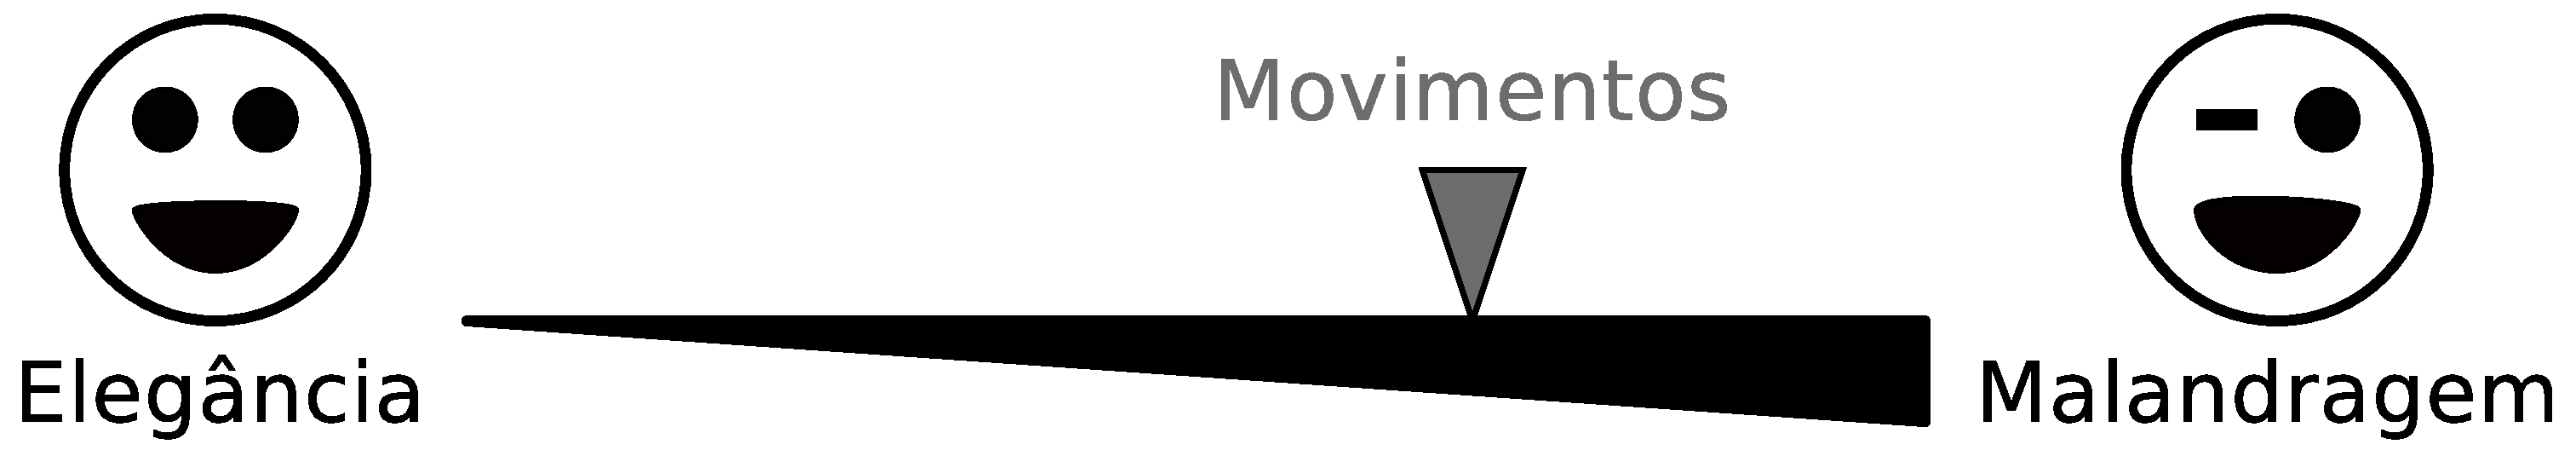
\includegraphics[width=0.65\textwidth]{chapters/cap-musicalidade/malandragem-elegancia.eps}
\caption{Malandragem e elegância.}
\label{fig:malandragem-elegancia}
\end{figure}


%%%%%%%%%%%%%%%%%%%%%%%%%%%%%%%%%%%%%%%%%%%%%%%%%%%%%%%%%%%%%%%%%%%%%%%%%%%%%%%%
\subsection{Dinâmica: Velocidade }
\label{subsec:dinamica:velocidade}
\index{Musicalidade!Velocidade}


Podemos achar o fator do movimento, ``velocidade'', entre dois extremos: lento e  rápido.
Como foi mencionado nos casos anteriores, 
na maioria das vesses, 
quando dançamos desaproveitamos o fator velocidade usando só um valor intermédio,
variando  pouco ao redor deste valor.
Assim, uma forma de treinar a velocidade seria manter, na medida do possível,
os outros fatores como continuidade e força em valores intermediários,
para assim trabalhar levando a velocidade a seus extremos em nossas dinâmicas.

Não devemos esquecer que a velocidade (v) está relacionada com a distancia percorrida (d) e o tempo (t),
mediante a Equação \ref{eq:vdt}.
\begin{equation}
\label{eq:vdt}
v=\frac{d}{t}
\end{equation}
Assim, 
uma forma de alterar a velocidade é modificar coerentemente o percorrido ou a duração do movimento.


\begin{description}
\item[Lento:] Neste caso nossos movimentos terão uma velocidade abaixo da media.
Para diminuir a velocidade podemos tomar dois caminhos.
\begin{itemize}
\item O primeiro seria manter constante a distancia do percorrido de nosso movimento,
e aumentar o tempo que empregamos para realizar este.
\item O segundo seria manter constante a duração do movimento e diminuir a distancia percorrida por este. 
\end{itemize}
\item[Rápido:] Por oposição ao caso anterior, 
aqui nossos movimentos estarão acima da media.
Para aumentar a velocidade podemos tomar dois caminhos.
\begin{itemize}
\item O primeiro seria manter constante a distancia do percorrido de nosso movimento,
e diminuir o tempo que empregamos para realizar este.
\item O segundo seria manter constante a duração do movimento e aumentar a distancia percorrida por este. 
\end{itemize}
\end{description}

\begin{example}[Treinando mantendo constante o tempo:]
Para este treinamento devemos escolher uma música, por exemplo uma em compasso binário,
identificar o tempo forte e fraco, e logo executar nossos movimentos em cada tempo,
de modo que o único que podemos modificar em nossas dinâmicas seja a distancia percorrida,
e consequentemente a velocidade da dinâmica, que estará em função de algum aspecto da música.
Uma possível escolha de movimento seria dar passos a alguma direção.
\end{example}

\begin{example}[Treinando mantendo constante a distancia:]
Para este treinamento devemos realizar movimentos com o mesmo percorrido,
e modificar o tempo que utilizamos para executar ele, 
de modo que indiretamente modifiquemos a velocidade da dinâmica.

Assim, para este treino devemos fazer marcas equidistantes, fisicamente ou mentalmente, 
sobre uma superfície, 
e interpretaremos uma música só nos movimentando de uma marca a outra,
de modo que seja o tempo do percorrido o único fator que modifiquemos.
\end{example}


\begin{example}[Velocidade constante no ``tchic tchic tum'':]~

\begin{abc}[name=abc-veltchictchictum,width=0.38\textwidth]
X: 1 % start of header
K: C stafflines=1 % scale: C major
M: 2/4 %meter - compasso
%Q:1/4=80
V:1 clef=perc stem=up %name="Pauta com clave de fá"   sname="Pauta com clave de fá"
[V:1] |: B2 B1 B1:|
w: tum tchic tchic
\end{abc}

Um treinamento interessante para desenvolver o contro corporal,
pode ser feito utilizando uma sequencia rítmica  ``tchic tchic tum''.
Neste caso tentaremos manter uma velocidade constante em nosso andar,
enquanto nossos pés executam passos com cada som, já seja um ``tchic'' ou um ``tum''.

Observem que o tempo de nossos movimentos é fixo e definido pela sequencia rítmica,
porém este é irregular, tendo um tempo de reação dobrado para o movimento apos ``tum'',
que para os movimentos apos um ``tchic''.
Assim, com essa distribuição irregular de tempos, 
devemos também ter uma distribuição  irregular de distancias de percorrido,
para poder manter constante a velocidade de nosso movimento.
\end{example}
%: ``slow motion'' e velocidade aumentada




%%%%%%%%%%%%%%%%%%%%%%%%%%%%%%%%%%%%%%%%%%%%%%%%%%%%%%%%%%%%%%%%%%%%%%%%%%%%%%%%
\subsection{Dinâmica: Energia }
\label{sec:musicalidadenergia}
O fator do movimento ``energia'', 
tem níveis  que vão entre dois extremos: baixa e alta energia.
Nos seguintes exercícios, quantificaremos esta faixa de energia em só 3 neveis,
que usaremos para mostrar texturas em nossos movimentos.

\begin{figure}[!h]
  \centering
    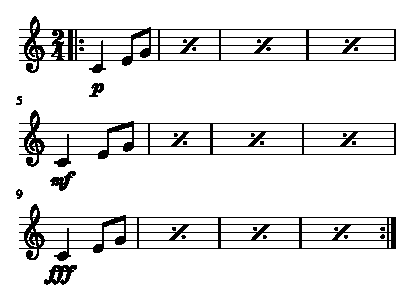
\includegraphics[width=0.65\textwidth]{chapters/cap-musicalidade/dinamica-energia-1.eps}
\caption{Ritmos usando 3 distintos matizes nas dinâmicas.}
\label{fig:dinamica-energia-ex1}
\end{figure}

\begin{example}[Usando 3 níveis de energia: sem deslocamento]
Para realizar este exercício, escolheremos um movimento; como por exemplo,
pisar no lugar, com um pé por vez, 
e com nosso movimento  acompanharemos nota por nota 
ao ritmo descrito na pauta da Figura \ref{fig:dinamica-energia-ex1}.
\begin{itemize}
\item Quando o ritmo tenha um matiz ``piano'' (\textbf{\textit{p}}) 
usaremos um movimento com suave,
com pouca força e quase sem movimentar-nos.
\item Quando o ritmo tenha um matiz ``mezzo forte'' (\textbf{\textit{mf}}) 
usaremos um movimento que seja natural e cotidiano,
com uma força regular, movimentando-nos de forma relaxada.
\item Quando o ritmo tenha um matiz ``extremadamente forte''  (\textbf{\textit{fff}}) 
usaremos um movimento que seja exagerado,
com uma muita força com movimentos como atacando o chão.
\end{itemize}
\end{example}

\begin{example}[Usando 3 níveis de energia: com deslocamento]
Para realizar este exercício, escolheremos um movimento; como por exemplo,
dar um passo, com um pé por vez, 
e com nosso movimento acompanharemos nota por nota 
ao ritmo descrito na pauta da Figura \ref{fig:dinamica-energia-ex1}.
\begin{itemize}
\item Quando o ritmo tenha um matiz ``piano'' (\textbf{\textit{p}}) 
daremos um passo extremadamente curto e suave como se tivéssemos medo de quebrar o chão.
\item Quando o ritmo tenha um matiz ``mezzo forte'' (\textbf{\textit{mf}}) 
daremos um passo de andar natural, com uma força regular e um passo relaxado. 
\item Quando o ritmo tenha um matiz ``extremadamente forte''  (\textbf{\textit{fff}}) 
daremos passos muitos longos, com muita energia no nosso andar, 
procurando recorrer a maior distancia possível.
\end{itemize}
\end{example}

\begin{FraseFernandoPR}{Causa-efeito}
Algumas vezes você tem que \hyperref[ref:emotionsentimental]{\textbf{sentir-se}} feliz para poder sorrir,
porém outras vezes você terá que sorrir para poder chegar a sentir-se feliz. %(2018-03-30)
\end{FraseFernandoPR}

